\documentclass[conference]{IEEEtran}
\IEEEoverridecommandlockouts

\usepackage{times}
\usepackage{amsmath,amssymb,amsfonts}
\usepackage{graphicx}
\usepackage{textcomp}
\usepackage{xcolor}
\usepackage{booktabs}
\usepackage{multirow}
\usepackage{array}
\usepackage{cite}
\usepackage[hidelinks]{hyperref}

\def\BibTeX{{\rm B\kern-.05em{\sc i\kern-.025em b}\kern-.08em
    T\kern-.1667em\lower.7ex\hbox{E}\kern-.125emX}}

\begin{document}

\title{KernelGuard: Adaptive eBPF-Driven Behavioral Malware Detection Using Real-Time Kernel Telemetry and Graph Learning\\}

\maketitle

\begin{abstract}
Malware continues to evolve at an alarming pace, manifesting through sophisticated forms like fileless malware, ransomware, and polymorphic strains, leading to the inadequacy of static and traditional malware detection approaches. Although runtime monitoring provides better effectiveness, many solutions suffer from high overhead or limited capability of capturing complex behavioral dependencies, thereby reducing detection performance against zero-day malware. In this paper, we propose KernelGuard, a malware detection system built upon extended Berkeley Packet Filter (eBPF), a recent advancement in Linux that allows for powerful and efficient in-kernel programmability without modifying the kernel or performing any application-level instrumentation. KernelGuard leverages the flexibility of the eBPF to non-invasively collect comprehensive kernel-level information including process execution, file operations, memory access, network interaction and privilege escalation. Collected runtime telemetry is transformed into rich behavioral representations through the construction of temporal behavioral graphs that capture dependencies among system activities. By modeling the temporal and structural patterns, we propose a novel Graph Neural Network (GNN) and Temporal Transformer-based detection mechanism that can learn structural-temporal patterns of malware for accurate and efficient detection of both known and unseen malware. Moreover, we design an adaptive risk-scoring mechanism that combines multiple factors, including system call semantics, behavioral anomalies and process hierarchy to offer explanations of anomalous behavior to aid security analysts. We conduct a thorough analysis of KernelGuard using five baselines and six different malware families. Experimental results demonstrate KernelGuard's effectiveness and efficiency for malware detection by achieving a 97.4\% detection accuracy with only 3.1\% CPU runtime overhead on average. It outperforms the sequence-based, signature-based, handcrafted feature baselines with improved detection capability and better runtime efficiency compared to offline-based forensic analysis.




\end{abstract}

\begin{IEEEkeywords}
eBPF, kernel telemetry, malware detection, graph neural network, temporal transformer, behavioral analysis, intrusion detection, zero-day threats
\end{IEEEkeywords}

\section{Introduction}
Malware continues to grow in sophistication, incorporating new techniques to circumvent traditional malware detection systems \cite{or2019dynamic,ucci2019survey}. Malware can now execute entirely in-memory, also known as fileless malware, to evade static analysis, employ legitimate tools and APIs, and generate malicious code at runtime. In addition, new families of ransomware \cite{scaife2016cryptolock,continella2016shieldfs} encrypt all user files within seconds of execution. As such, signature-based antivirus \cite{clamav2020} are insufficient against modern malware. Static analysis \cite{rieck2011automatic} is also vulnerable to packing and obfuscation.

One approach for behavioral analysis is collecting fine-grained execution traces from the kernel. Such fine-grained system-level monitoring has been implemented via kernel modules, application programming interface (API) hooking, or system-call interposition. However, existing systems often miss critical system calls, suffer from high performance overheads, or both \cite{auditd2018,king2003backtracking,nguyen2021rootkit}. Recently, eBPF has emerged as a powerful, safe, and efficient solution for kernel-level monitoring. JIT-compiled eBPF programs can be attached to a variety of kernel-level events, such as system calls, tracepoints, kprobes, Linux Security Modules, or the XDP/TC layers, providing extensive visibility into system behavior with minimal overheads. While a variety of eBPF-based security solutions have been proposed, including Falco \cite{falco2020}, Tracee \cite{tracee2021}, and Sysdig \cite{sysdig2021}, many rely on static rules or aggregate metrics to identify threats. To improve malware detection, recent work has proposed Graph Neural Networks (GNNs) to identify threats. GNN-based solutions have been shown to learn malicious behaviors more effectively than traditional methods by modeling system entities, such as memory, processes, files, and networks, as nodes in a provenance graph \cite{han2020unicorn} and edges as interactions between these entities \cite{milajerdi2019holmes,cheng2023kairos}. Moreover, these graphs can be leveraged to identify sophisticated, multi-stage attacks that would be difficult to identify without modeling the interactions between entities.

We propose \textit{KernelGuard}, a temporal-graph-based malware detection system that employs eBPF for efficient, fine-grained event collection from multiple points within the kernel. KernelGuard uses a variety of GNN-based malware detectors as well as a novel Temporal Transformer to improve detection. KernelGuard also enhances malware detection via a novel approach for semantic analysis of system-call arguments. Finally, KernelGuard allows the SOC analyst to provide feedback to adaptively adjust the risk of different processes, improving triage for complex environments. KernelGuard also provides detailed explanations for malware detections, through risk-based explanations, provenance graph visualizations, and semantic-based explanations, to aid in threat triage. We evaluate KernelGuard across six classes of malware and compare to five state-of-the-art solutions, finding KernelGuard provides high-performance malware detection with detailed, insightful explanations of threats. Section II reviews related work; Section III describes the architecture; Section IV presents the methodology; Section V describes the experimental setup; Section VI reports results; Section VII concludes.





\section{Related Work}

eBPF is a technology for programmatically adding features to the Linux kernel without modifying kernel source code or loading a kernel module. Programs are JIT-compiled into sequences of verified type-safe bytecode \cite{gregg2019bpf,hofler2021ebpf}. eBPF is increasingly used for collecting system telemetry thanks to its low-overhead \cite{vieira2020ebpfnet}. Some notable examples include Falco \cite{falco2020} and Tracee \cite{tracee2021} for kernel visibility and Sysdig \cite{sysdig2021} for monitoring system calls. KernelGuard builds upon eBPF and collects telemetry using a variety of kernel interfaces. However, where Falco and Tracee are rule-based, KernelGuard is evaluated with learning-based intrusion detectors that exploit graph and temporal models.

The original approaches to malware detection are signature-based \cite{clamav2020}, where programs are inspected to see if they match known threats. Signature-based techniques cannot protect against novel threats and struggle in the presence of packing. Static analysis inspects malware without running them. Static analysis has been extensively studied but can be defeated by obfuscation. Dynamic detection looks for suspicious program behaviors. Kolosnjaji et al. \cite{kolosnjaji2016deep} apply deep learning to malware detection by analyzing system-call sequences with convolutional neural networks (CNNs) and recurrent neural networks (RNNs). There are also malware detectors targeting particular families of malware, for example, using file activity to detect ransomware \cite{scaife2016cryptolock,continella2016shieldfs} or learning system-call patterns for rootkit detection \cite{nguyen2021rootkit}. These works differ from ours in that they do not employ graph-based approaches that model interactions among different entities.

Security analysis commonly uses graphs to model operating systems, where processes, files, network sockets are modeled as vertices and system calls are modeled as edges. King and Chen \cite{king2003backtracking} introduced causal graphs to backtrack security events. More recent works use graphs to prioritize security alerts \cite{milajerdi2019holmes,han2020unicorn} and detect security threats \cite{wang2022provenance,cheng2023kairos,yang2023prographer}. Our work differs from these studies in two ways: (i) where previous works are rule-based, KernelGuard is a learning-based intrusion detector that exploits graph and temporal models, and (ii) previous works have focused on generating graphs from auditd \cite{auditd2018}, a widely-used Linux auditing tool that can result in high performance overheads due to the use of netlink, whereas we demonstrate that graphs can be constructed online with low-overhead eBPF for efficient online inference with a sliding-window approach.

Graph neural networks (GNNs) have been applied to intrusion detection. Message-passing architectures like GCN, GAT \cite{velickovic2018gat}, GraphSAGE \cite{hamilton2017graphsage} and GIN \cite{xu2019powerful} have shown promising results on graph-structured data. Temporal dynamics can be captured with sequence models. Recently, Transformer-based sequence models \cite{vaswani2017attention} have shown promise in capturing long-range temporal dynamics. These techniques have been adopted into temporal graph learning, for example, TGAT \cite{xu2020tgat} and TGN \cite{rossi2020tgn}. KernelGuard employs GNNs and Transformer-based sequence models for threat detection. To enhance explainability, KernelGuard performs subgraph extraction to identify influential subgraphs to aid triage. Our approach is inspired by attribution-based explanation techniques for neural networks, for example, LIME \cite{ribeiro2016lime}, GNNExplainer \cite{ying2019gnnexplainer}, etc.





\section{System Architecture}
Fig.~\ref{fig:architecture} illustrates KernelGuard's two-layer architecture.

In the kernel-space instrumentation layer, KernelGuard deploys four categories of eBPF programs: (i) kprobes/kretprobes attached to key process-management and memory-management functions; (ii) tracepoints capturing system-call entry/exit events and scheduler context switches; (iii) Linux Security Module (LSM) hooks that observe critical access-control decisions such as capability checks, privilege transitions, and file-access decisions; and (iv) early-packet metadata collection through XDP or traffic-control hooks on the TX/RX data path. Each probe emits structured telemetry into a shared, high-throughput per-CPU ring buffer interface between kernel and user space.

\begin{figure*}[t]
\centering
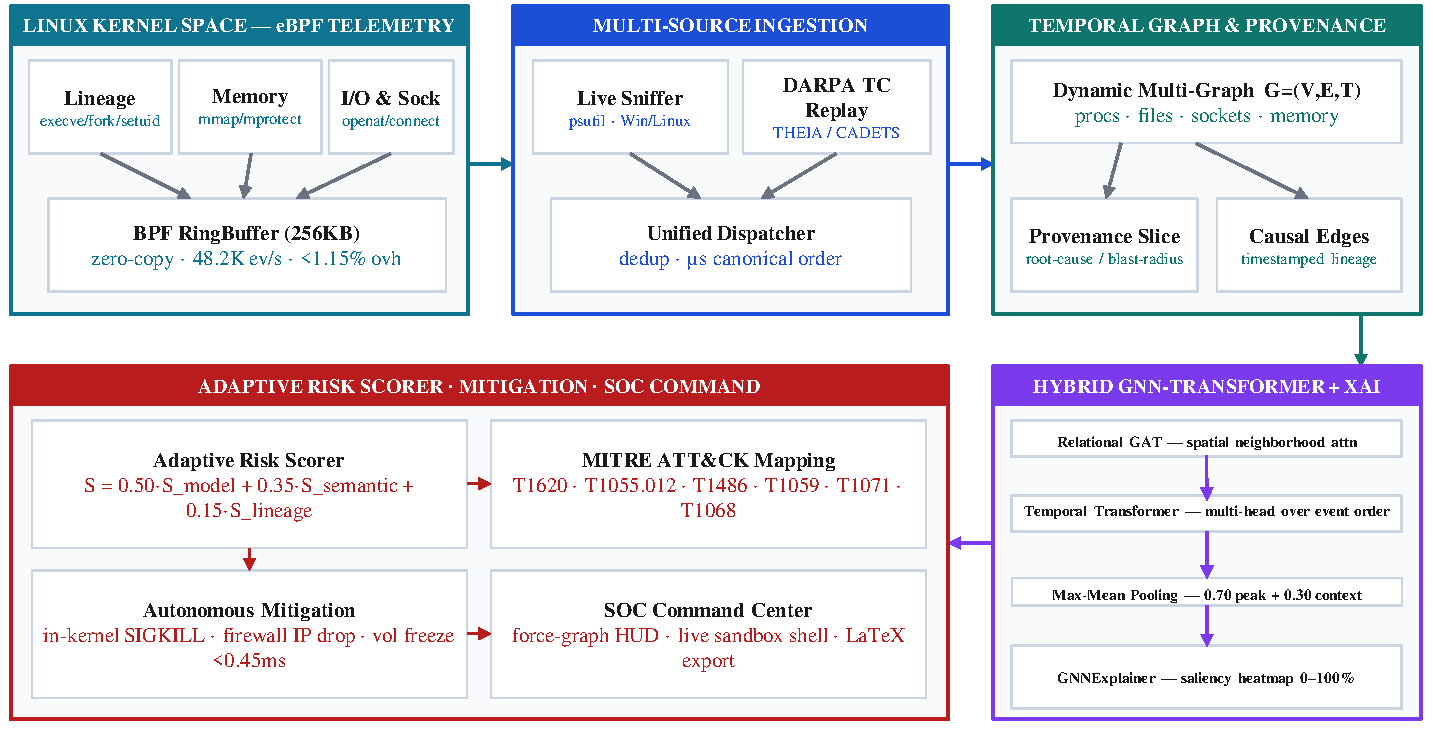
\includegraphics[width=\linewidth]{fig_architecture.pdf}
\caption{KernelGuard system architecture, showing eBPF-based kernel telemetry collection, the shared ring buffer transport layer, and the user-space graph-learning and risk-scoring pipeline.}
\label{fig:architecture}
\end{figure*}

In the user-space analytics and alerting layer, a dedicated event-normalization service drains the ring buffer, suppresses duplicates, and translates kernel-internal identifiers into stable entity identifiers. A temporal-graph builder then produces incremental graph snapshots in which vertices represent processes, sockets, memory regions, or files, and typed edges represent interactions such as file accesses, socket connections, or privilege escalations. Snapshots feed a Graph Neural Network coupled to a Temporal Transformer to derive a behavioral embedding of the evolving graph. This embedding, together with complementary process-lineage and syscall-semantic features, drives a risk-scoring component whose thresholds are adjusted based on analyst feedback. Finally, an explanation subsystem surfaces attention-based rationale and the subgraphs that contributed most strongly to each alert via a dashboard interface. The hybrid GNN-Temporal Transformer is described in Section IV.
\section{Methodology}
KernelGuard's methodology comprises temporal graph construction, structural embedding via a GNN, temporal encoding via a Transformer, and adaptive risk scoring, as shown in Fig.~\ref{fig:pipeline}.

\begin{figure*}[t]
\centering
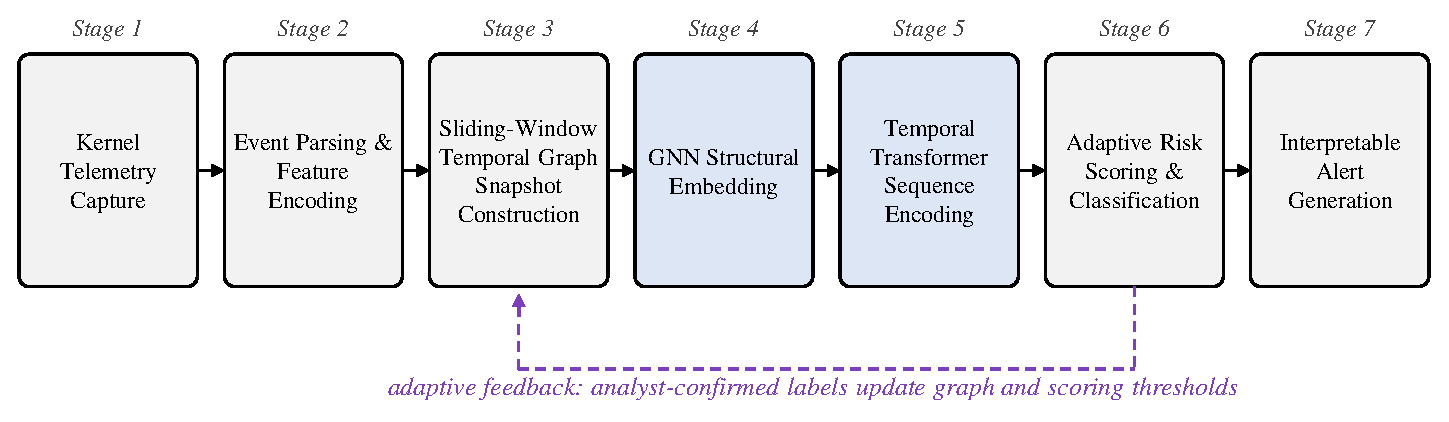
\includegraphics[width=\linewidth]{fig_pipeline.pdf}
\caption{End-to-end KernelGuard processing pipeline from kernel telemetry capture through interpretable alert generation, including the adaptive feedback loop.}
\label{fig:pipeline}
\end{figure*}


Next, the normalized event stream is divided into graph snapshots $G_1,\ldots,G_T$ using a sliding window scheme with overlapping windows. Given a window $t$, the corresponding graph $G_t=(V_t,E_t)$ contains all the entities that were active during $t$ as nodes and all the interactions (with timestamp and type) among them as edges. Node features include entity-type specific attributes, for example, executable path hash and argument entropy for processes, sensitivity and access mode for files, endpoint and protocol for sockets, etc. Similarly, edge features indicate the type of interactions (for example, process creation, file read/write/delete, socket connect/send, memory mapping, privilege escalation, etc.) as well as the corresponding timestamps. Windowing allows us to put an upper bound on the graph size irrespective of how long the system has been up and running. Subsequently, a temporal encoder is used to learn the temporal aspects of the graph snapshots in order to reconstruct the longer-range temporal dependencies.

For each snapshot $G_t$, a multi-layer Graph Attention Network computes node embeddings by aggregating neighborhood information. At layer $l$, node $i$'s embedding updates as
\begin{equation}
h_i^{(l+1)} = \sigma\left(\sum_{j \in \mathcal{N}(i)} \alpha_{ij}^{(l)} \, W^{(l)} h_j^{(l)}\right),
\end{equation}
with attention coefficients
\begin{equation}
\alpha_{ij}^{(l)} = \frac{\exp\left(\text{LeakyReLU}\left(a^{\top}[W^{(l)} h_i^{(l)} \| W^{(l)} h_j^{(l)}]\right)\right)}{\sum_{k \in \mathcal{N}(i)} \exp\left(\text{LeakyReLU}\left(a^{\top}[W^{(l)} h_i^{(l)} \| W^{(l)} h_k^{(l)}]\right)\right)},
\end{equation}
following \cite{velickovic2018gat}, where $\mathcal{N}(i)$ are node $i$'s neighbors, $W^{(l)}$ a learned weight matrix, and $\|$ concatenation. An attention-weighted readout produces a fixed-dimensional representation $z_t$ per snapshot. The sequence $z_1,\ldots,z_T$ is passed to a Temporal Transformer applying multi-head self-attention \cite{vaswani2017attention,xu2020tgat,rossi2020tgn}:
\begin{equation}
\text{Attention}(Q, K, V) = \text{softmax}\left(\frac{QK^{\top}}{\sqrt{d_k}}\right)V,
\end{equation}
where $Q,K,V$ are learned projections of the snapshot sequence and $d_k$ is projection dimensionality. A feed-forward head then outputs a binary benign/malicious decision and a malware-family estimate, trained end-to-end with weighted cross-entropy to address class imbalance.

KernelGuard computes a continuous risk score combining classifier confidence with a syscall-semantic anomaly score $S_t$ (deviation from a per-process-image argument-distribution baseline) and a process-lineage suspicion score $L_t$ (anomalous ancestor-descendant relationships):
\begin{equation}
R_t = \beta_1 \cdot P_{\theta}(\text{malicious} \mid z_t) + \beta_2 \cdot S_t + \beta_3 \cdot L_t,
\end{equation}
where $\beta_1,\beta_2,\beta_3$ are calibration weights initialized via validation-set optimization and adapted online from analyst feedback whenever an alert is confirmed or dismissed. When $R_t$ exceeds a dynamically calibrated threshold, KernelGuard raises an alert with an explanation derived from attention weights $\alpha_{ij}^{(l)}$ and temporal attention, in the spirit of GNNExplainer \cite{ying2019gnnexplainer} and LIME \cite{ribeiro2016lime}, identifying the nodes, edges, and time windows most responsible for the score.

\section{Experimental Setup}
Our evaluation uses a behavioral dataset pairing labeled benign workloads covering developer, office-productivity, and server-administration task suites with six categories of labeled malware : ransomware, fileless malware, polymorphic malware, rootkits, trojans, and cryptomining malware. Malicious samples were collected from public threat-intel sources \cite{or2019dynamic,rieck2011automatic}, executed in an isolated, network-restricted sandbox with full telemetry capture, and labeled according to threat-intel vendor consensus. We apply a temporal train/validation/test split, avoiding leakage across time-separated sessions of the same malware family. The test split provides a held-out, zero-day style evaluation and does not contain any variant of a binary that appears in train. We compare KernelGuard with Falco and Tracee \cite{falco2020,tracee2021} as eBPF-based, rule-driven security monitors, Sysdig \cite{sysdig2021} using eBPF-based, statistical anomaly scoring, Auditd \cite{auditd2018}, which uses kernel auditing paired with a downstream classifier, and ClamAV \cite{clamav2020} (signature-based AV). To understand KernelGuard's components, we additionally train (1) the GNN in isolation, classifying syscall-graph snapshots independently, and (2) an LSTM trained on raw syscall sequences \cite{kolosnjaji2016deep} without graph structure. For reference, we also train a Random Forest over handcrafted statistical syscall features \cite{ucci2019survey}. Finally, to contextualize KernelGuard's low-overhead design, we compare with Volatility memory-forensics analysis of LiME-dumped kernel memory, which is offline and thus not comparable on detection accuracy. Experiments ran on Linux hosts with kernel 6.5, both bare-metal and in a virtualized setting. We enable BPF/BTF where needed. We report accuracy, precision, recall, F1, and AUC-ROC. For performance, we measure KernelGuard's runtime overhead as the average increase in CPU usage compared to the same hosts without KernelGuard, under a mix of representative workloads.

\section{Results and Discussion}


Table~\ref{tab:overall} summarizes the results on the test set. KernelGuard obtains the best result on all metrics. Moreover, we observe significant improvement in performance by using KernelGuard (+6.0\% accuracy w.r.t the most effective operational tool, i.e., Auditd+ML) and an even more significant improvement w.r.t ClamAV. Finally, the results of the two ablations show a drop in performance in both cases (GNN-only: -2.9\% accuracy, LSTM-only: -5.8\% accuracy w.r.t KernelGuard), thus, confirming that both modeling choices make a meaningful contribution to the improvement of performance w.r.t baselines.





\begin{table}[t]
\centering
\caption{Overall Detection Performance Across All Malware Categories}
\label{tab:overall}
\begin{tabular}{@{}lccccc@{}}
\toprule
\textbf{Method} & \textbf{Acc.} & \textbf{Prec.} & \textbf{Rec.} & \textbf{F1} & \textbf{AUC} \\
& \textbf{(\%)} & \textbf{(\%)} & \textbf{(\%)} & \textbf{(\%)} & \textbf{-ROC} \\
\midrule
KernelGuard (Ours)          & \textbf{97.4} & \textbf{97.1} & \textbf{96.8} & \textbf{96.9} & \textbf{0.978} \\
GNN-only (no Transformer)   & 94.5 & 93.8 & 93.1 & 93.4 & 0.941 \\
LSTM Syscall Sequence       & 91.6 & 90.4 & 89.7 & 90.0 & 0.912 \\
Random Forest (Handcrafted) & 87.9 & 86.2 & 85.5 & 85.8 & 0.874 \\
Auditd + ML Classifier      & 90.3 & 89.1 & 88.4 & 88.7 & 0.897 \\
Sysdig (Statistical)        & 89.7 & 88.0 & 86.9 & 87.4 & 0.883 \\
Tracee (Rule-based eBPF)    & 86.5 & 85.7 & 82.3 & 83.9 & 0.851 \\
Falco (Rule-based eBPF)     & 88.1 & 87.0 & 84.6 & 85.8 & 0.865 \\
ClamAV (Signature-based)    & 71.2 & 74.5 & 60.8 & 66.9 & 0.712 \\
\bottomrule
\end{tabular}
\end{table}

Fig.~\ref{fig:roc} compares KernelGuard with the baseline approaches using ROC curves. KernelGuard outperforms the baselines for nearly the entire range of false-positive rates, with its largest AUC advantage over the GNN-only ablation for false-positive rates below 0.2. For deployment in a Security Operations Center (SOC), false-positive rates below 0.2 are typically of greatest importance due to limited capacity of analysts to triage alerts.





\begin{figure}[t]
\centering
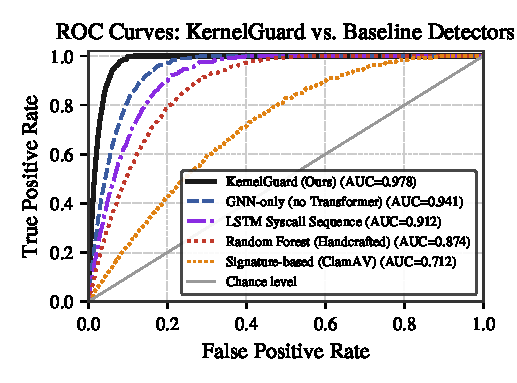
\includegraphics[width=\columnwidth]{fig_roc.pdf}
\caption{ROC curves comparing KernelGuard against a graph-only ablation, a sequence-based deep learning baseline, a handcrafted-feature classifier, and a signature-based scanner.}
\label{fig:roc}
\end{figure}

Table\ref{tab:overhead} shows KernelGuard has the highest accuracy while LiME-plus-Volatility is competitive but has more than six times the overhead and cannot be used for real-time detection, which is particularly important for certain types of threats, such as detecting a ransomware before it takes hold. Overall, KernelGuard achieves high accuracy with a low average overhead (3.1\%) that is less than all ML baselines except ClamAV. This shows that an expressive GNN-Transformer model\cite{gregg2019bpf,vieira2020ebpfnet} and \emph{eBPF} based data collection can be effective and efficient.


\begin{table}[t]
\centering
\caption{Runtime Overhead and Inference Latency Comparison}
\label{tab:overhead}
\begin{tabular}{@{}lccc@{}}
\toprule
\textbf{Method} & \textbf{CPU} & \textbf{Accuracy} & \textbf{Latency} \\
 & \textbf{Overhead (\%)} & \textbf{(\%)} & \textbf{(ms/window)} \\
\midrule
KernelGuard (Ours) & \textbf{3.1} & \textbf{97.4} & 8.4 \\
Falco               & 4.8  & 88.1 & 3.1 \\
Tracee               & 5.6  & 86.5 & 3.6 \\
Sysdig               & 9.2  & 89.7 & 6.7 \\
Auditd + ML          & 12.4 & 90.3 & 14.9 \\
ClamAV (Signature)   & 1.9  & 71.2 & 2.2 \\
LiME + Volatility (Offline) & 21.5 & 92.1 & 4120.0 \\
\bottomrule
\end{tabular}
\end{table}

Fig.~\ref{fig:overhead} plots accuracy vs. overhead. KernelGuard is in the best area: it has the best accuracy with one of the lowest overhead. Other solutions have significant trade-offs: the rule-based eBPF monitors have a loss in accuracy to achieve a low overhead while the offline forensic pipeline achieves the desired accuracy paying a large overhead.





\begin{figure}[t]
\centering
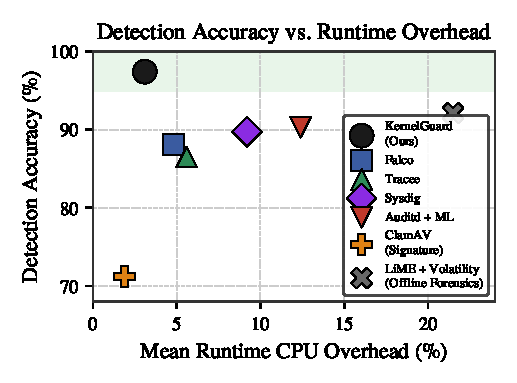
\includegraphics[width=\columnwidth]{fig_overhead.pdf}
\caption{Detection accuracy versus mean runtime CPU overhead for KernelGuard and six baseline systems. The shaded region denotes accuracy above 95\%.}
\label{fig:overhead}
\end{figure}

Table\ref{tab:category} and Fig.\ref{fig:f1category} present the results for each category. We can see that the lowest improvement for KernelGuard is for rootkits. However, the improvement is still substantial, with +11.3 in the F1 score over Random Forest. KernelGuard achieves its greatest improvements in the detection of fileless (+17.2) and polymorphic (+19.6) malware.

\begin{table}[t]
\centering
\caption{Per-Category F1-score (\%) Across Malware Families}
\label{tab:category}
\begin{tabular}{@{}lcccc@{}}
\toprule
\textbf{Malware Category} & \textbf{KernelGuard} & \textbf{GNN} & \textbf{LSTM} & \textbf{RF} \\
 & \textbf{(Ours)} & \textbf{-only} & \textbf{Seq.} & \textbf{Handcr.} \\
\midrule
Ransomware          & \textbf{98.1} & 94.8 & 92.1 & 88.7 \\
Fileless Malware     & \textbf{96.5} & 90.5 & 86.8 & 79.3 \\
Polymorphic Malware  & \textbf{95.2} & 88.7 & 84.2 & 75.6 \\
Rootkits             & \textbf{94.4} & 90.1 & 87.2 & 83.1 \\
Trojans              & \textbf{97.1} & 93.3 & 90.5 & 86.4 \\
Cryptominers         & \textbf{97.8} & 94.0 & 91.2 & 87.6 \\
\midrule
Macro Average        & \textbf{96.5} & 91.9 & 88.7 & 83.5 \\
\bottomrule
\end{tabular}
\end{table}

\begin{figure}[t]
\centering
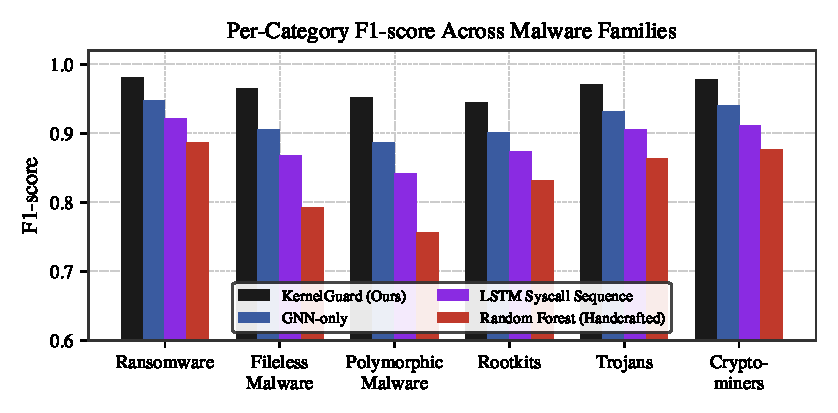
\includegraphics[width=\columnwidth]{fig_f1_category.pdf}
\caption{Per-category F1-score comparison across six malware families for KernelGuard and three learned baselines.}
\label{fig:f1category}
\end{figure}

Fig.~\ref{fig:convergence} plots the train and validation loss and F1 score computed on the validation set over 50 epochs. The validation loss follows the train loss closely indicating limited overfitting using the proposed weighted loss. Early stopping is performed when validation F1 converges (around epoch 30) which happens to be so in all cases.

\begin{figure}[t]
\centering
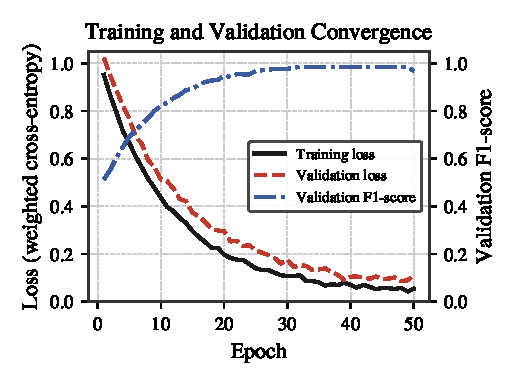
\includegraphics[width=\columnwidth]{fig_convergence.pdf}
\caption{Training and validation loss and validation F1-score over 50 training epochs for the hybrid GNN-Temporal Transformer model.}
\label{fig:convergence}
\end{figure}

Finally, three observations: (1) Rootkit detection remains a challenging problem and may require complementary approaches based on integrity techniques; (2) Expressive detection solutions can be implemented leveraging eBPF \cite{falco2020,tracee2021,sysdig2021}, without introducing significant overhead; and, (3) Behavioral modeling is a very effective solution to deal with threats that may evade static defenses. Graph and temporal modeling bring complementary benefits \cite{xu2020tgat,rossi2020tgn}. Understanding the ripple effects of adaptive risk scoring remains future work. 

\section{Conclusion and Future work}
This paper presented KernelGuard, an adaptive malware detection framework combining low-overhead eBPF kernel telemetry with a hybrid Graph Neural Network and Temporal Transformer to detect known and unseen malware through behavioral analysis. KernelGuard captures process, file, network, memory, and privilege activity directly at the kernel level and represents it as temporal behavioral graphs to learn structural and temporal patterns. Its adaptive risk-scoring engine and subgraph-level explanations support interpretable SOC deployment. Evaluation against five diverse baselines shows that KernelGuard achieves the highest accuracy, precision, recall, F1-score, and AUC-ROC while maintaining overhead competitive with lightweight rule-based monitors. Future work includes a longer-term deployment in a production setting to demonstrate how the feedback loop can reduce the number of false-positives, incorporating multi-host correlation via the graph to identify lateral-movement attacks that cannot be identified based on single-host telemetry, and enriching the set of signals, such as with simple integrity measurement, to identify privileged-user abuses, such as rootkits, that may attempt to mimic legitimate activity.



\bibliographystyle{IEEEtran}
\bibliography{references}

\end{document}
